\documentclass[11pt]{article}

\usepackage[margin=1in]{geometry}
\usepackage{graphicx}
\usepackage{booktabs}
\usepackage{float}
\usepackage{hyperref}
\usepackage{parskip}
\usepackage{caption}
\usepackage{xcolor}
\usepackage{tcolorbox}

\title{Slowloris Denial-of-Service Attack and Defense: \\ Evaluation Report}
\author{Afham Adian}
\date{\today}

\begin{document}

\maketitle

\section{Introduction}

This report documents a controlled experiment in which a web server was
subjected to a slow-connection denial-of-service attack, its impact was
measured, a defense was applied, and the same attack was repeated to
evaluate how effective that defense was.

The experiment involved three roles running at the same time:

\begin{itemize}
    \item a \textbf{legitimate user}, sending normal requests to the server
    at a steady rate throughout the whole test;
    \item an \textbf{attacker}, generating a large number of malicious
    slow connections during a fixed attack window;
    \item a \textbf{monitor}, continuously observing the server's health
    (how many of its connection slots were busy, CPU and memory usage).
\end{itemize}

Each test ran in three phases: a quiet \emph{baseline} period, an
\emph{attack} period, and a \emph{recovery} period after the attack
stopped. This was repeated at increasing attack sizes ($N = 20, 50, 100,
200$, where $N$ is the number of connections the attacker attempted to
open) so the effect of attack size could be observed directly. The server
was configured with a fixed maximum capacity of 30 concurrent
connections throughout every test, which is the key number this report's
results are measured against.

\section{The Attack}

\subsection{Steps of the Attack}

The attack works by exploiting how a web server holds a connection open
while it waits for a client to finish sending its request:

\begin{enumerate}
    \item The attacker opens a large number of connections to the server
    at once.
    \item On each connection, it sends just enough of a request to make
    it look valid and ongoing, but deliberately never finishes it.
    \item Every few seconds, it sends a small, harmless extra fragment on
    each connection, just enough to convince the server the client is
    still there and "about to finish," without ever actually
    completing the request.
    \item The server, following normal behaviour, keeps a connection slot
    reserved for each of these unfinished requests indefinitely, waiting
    for them to complete.
    \item Once enough connections are held open this way, the server has
    no free slots left for anyone else.
\end{enumerate}

Because each connection is trivial to open and keep alive, this lets a
single attacker with modest resources tie up far more server capacity
than its own resource usage would suggest.

\subsection{Victim-Side Snapshot}

To observe the effect directly, the attack was also demonstrated live,
following this sequence:

\begin{enumerate}
    \item Start the server.
    \item Open a client terminal.
    \item Send a request from the client to the server and confirm a
    normal response is received.
    \item Start the attacker.
    \item Send another request from the client terminal: it no longer
    receives a response.
\end{enumerate}

Figure~\ref{fig:victim-snapshot} shows the client terminal's output for
the last step: the request hangs until it hits its own timeout, instead
of getting a response from the server.

\begin{figure}[H]
\centering
\begin{tcolorbox}[colback=black!2, colframe=red!60!black, boxrule=1.2pt,
                   title=Victim-side terminal, fonttitle=\bfseries]
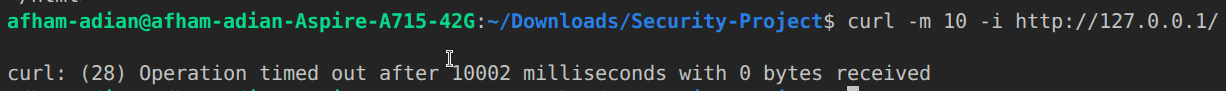
\includegraphics[width=0.85\textwidth]{figures/victim_curl_timeout.png}
\end{tcolorbox}
\caption{\textbf{After Attack:} client-side request sent while the
attack is running. The request times out with 0 bytes received instead
of getting a response.}
\label{fig:victim-snapshot}
\end{figure}

\subsection{Was the Attack Successful?}

Yes. Before the attacker was started, the same client request completed
normally, as shown in Figure~\ref{fig:victim-before}; once the attacker
was running, the identical request failed as shown earlier in
Figure~\ref{fig:victim-snapshot}.

\begin{figure}[H]
\centering
\begin{tcolorbox}[colback=black!2, colframe=green!45!black, boxrule=1.2pt,
                   title=Victim-side terminal, fonttitle=\bfseries]
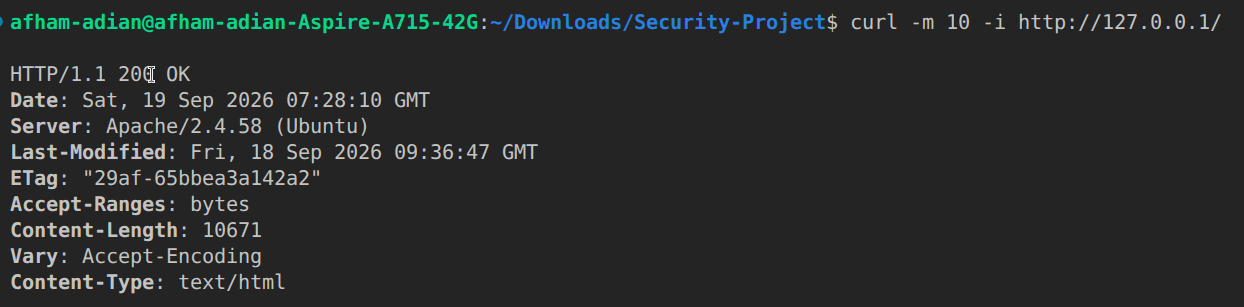
\includegraphics[width=0.85\textwidth]{figures/victim_curl_before_attack.png}
\end{tcolorbox}
\caption{\textbf{Before Attack:} the same client-side request sent
before the attacker was started, completing normally with an
HTTP 200 OK response.}
\label{fig:victim-before}
\end{figure}

Table~\ref{tab:attack-results} summarizes the legitimate user's
experience during the attack window at each attack size.

\begin{table}[H]
\centering
\caption{Legitimate client outcomes during the attack window, undefended server.}
\label{tab:attack-results}
\begin{tabular}{lllll}
\toprule
Attack size (N) & Client success rate & Avg.\ latency & Busy slots at peak & Result \\
\midrule
20  & 100\% & 0.09s & 23 / 30 & No denial \\
50  & 0\%   & 5.01s & 30 / 30 (exhausted) & Denial \\
100 & 0\%   & 5.01s & 30 / 30 (exhausted) & Denial \\
200 & 9\%   & 4.55s & 30 / 30 (exhausted) & Denial \\
\bottomrule
\end{tabular}
\end{table}

At $N = 20$, the attack had no visible effect: the server still had free
capacity, and the legitimate user's requests succeeded normally. From
$N = 50$ onward, the legitimate user's success rate collapsed to
effectively 0\%, and the few requests that did get through took roughly
5 seconds, the point at which the client simply gave up waiting.

\subsection{Why the Attack Was Successful}

The result lines up exactly with the server's fixed capacity of 30
concurrent connections. Below that threshold ($N = 20$), the attacker
could not occupy enough slots to crowd out the legitimate user. Once the
attack size passed that threshold ($N \geq 50$), every available slot
was taken up by an unfinished, deliberately-stalled connection, leaving
nothing for real traffic. The attack did not need to overwhelm the
server computationally: it only needed to exceed the number of
connection slots available, which is a comparatively small number and
easy to exceed with a modest number of attacking connections.

\subsection{Observed Output}

\begin{figure}[H]
\centering
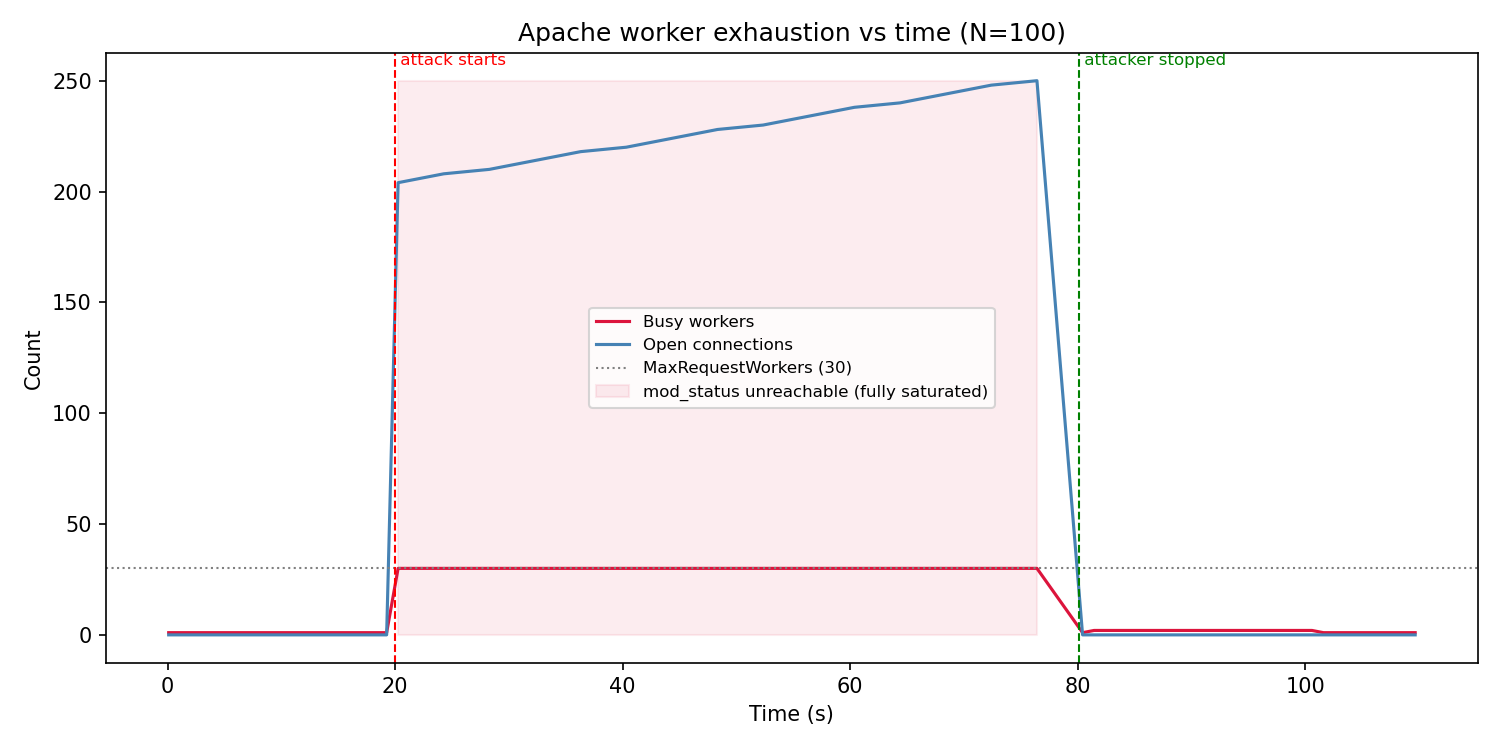
\includegraphics[width=0.85\textwidth]{../results/sweep_N100/1_worker_saturation.png}
\caption{Busy connection slots over time during the $N=100$ attack.
Occupied slots rise to the server's maximum during the attack window and
fall back afterward.}
\end{figure}

\begin{figure}[H]
\centering
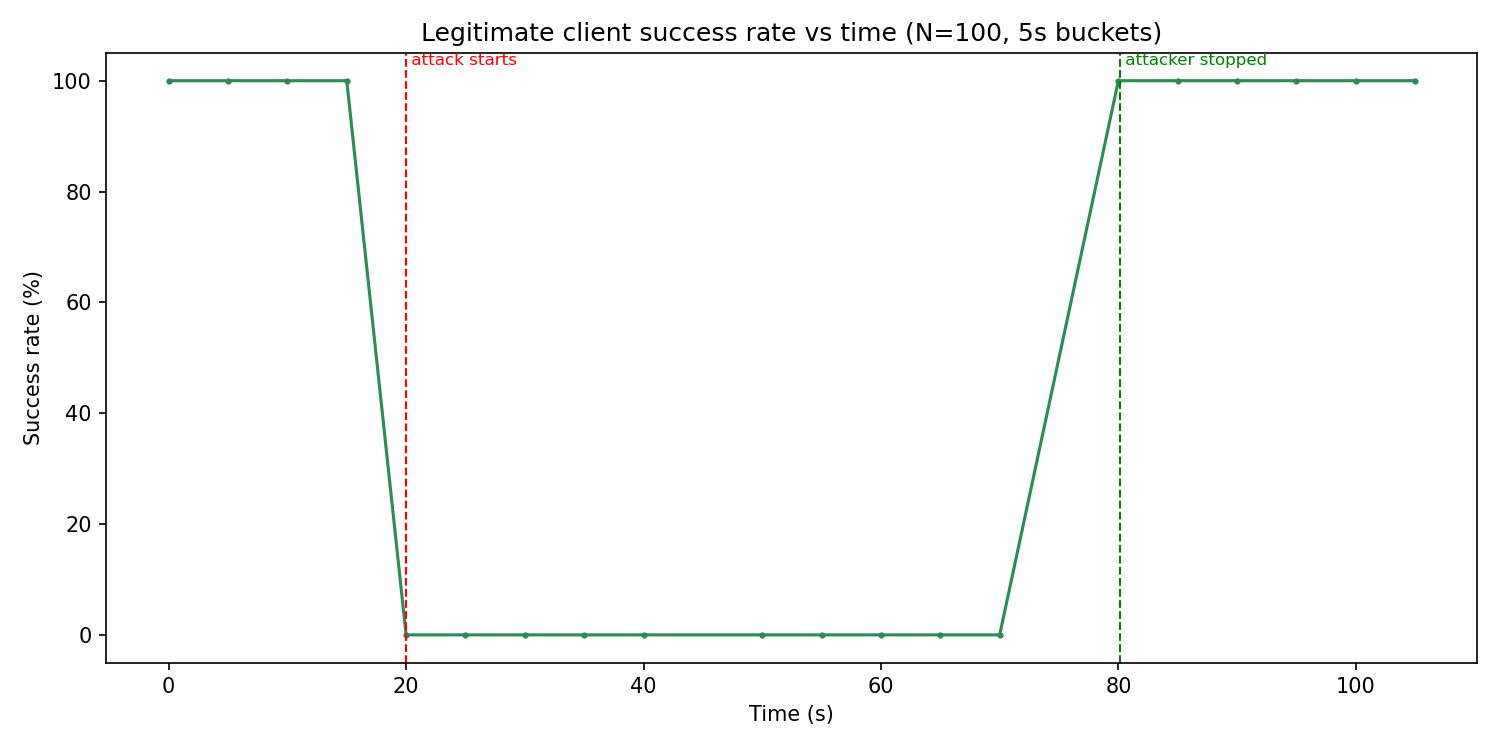
\includegraphics[width=0.85\textwidth]{../results/sweep_N100/3_client_success_rate.png}
\caption{Legitimate client success rate over time during the $N=100$
attack. Success drops to 0\% for the duration of the attack window and
recovers immediately once the attack stops.}
\end{figure}

\begin{figure}[H]
\centering
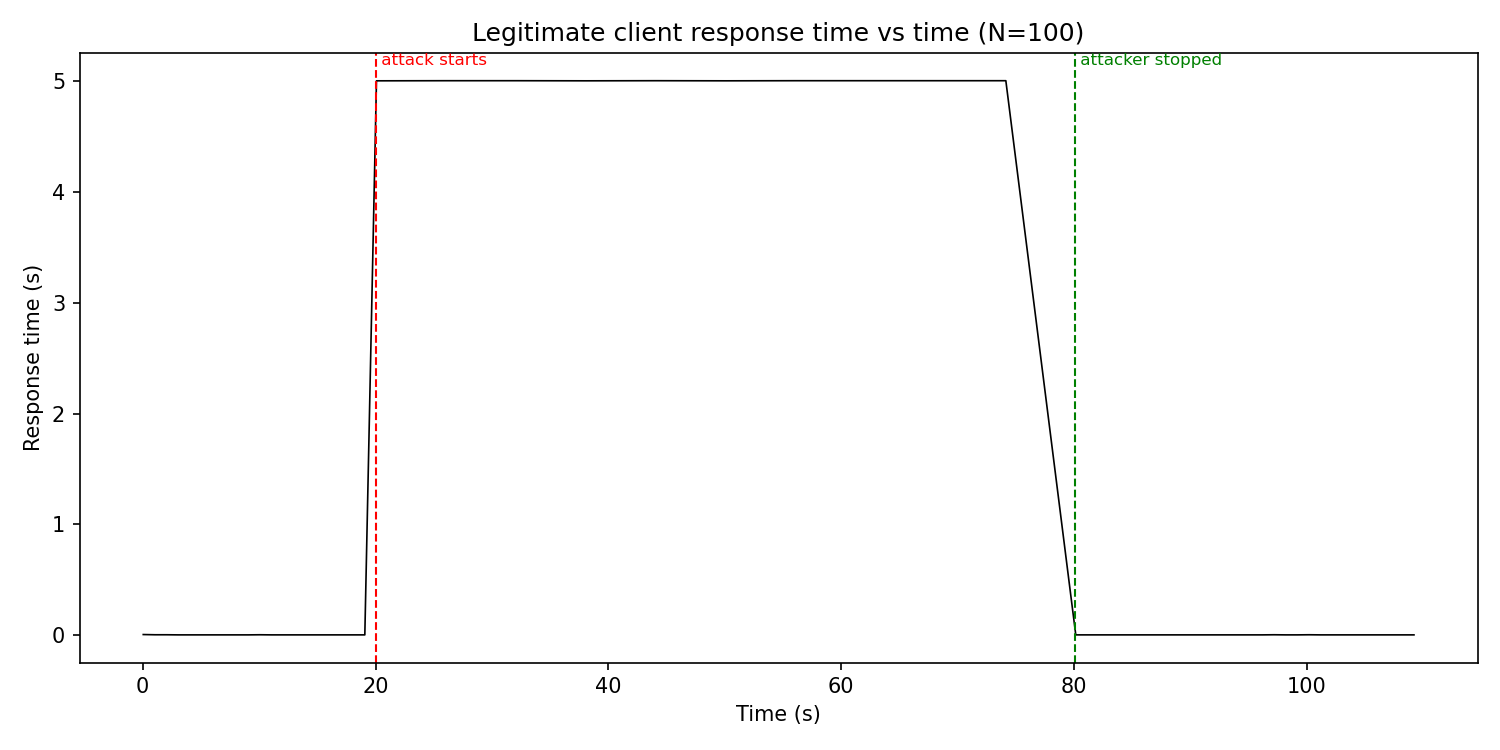
\includegraphics[width=0.85\textwidth]{../results/sweep_N100/4_client_latency.png}
\caption{Legitimate client response time over time during the $N=100$
attack, spiking to the client's own timeout ceiling for the duration of
the attack.}
\end{figure}

\begin{figure}[H]
\centering
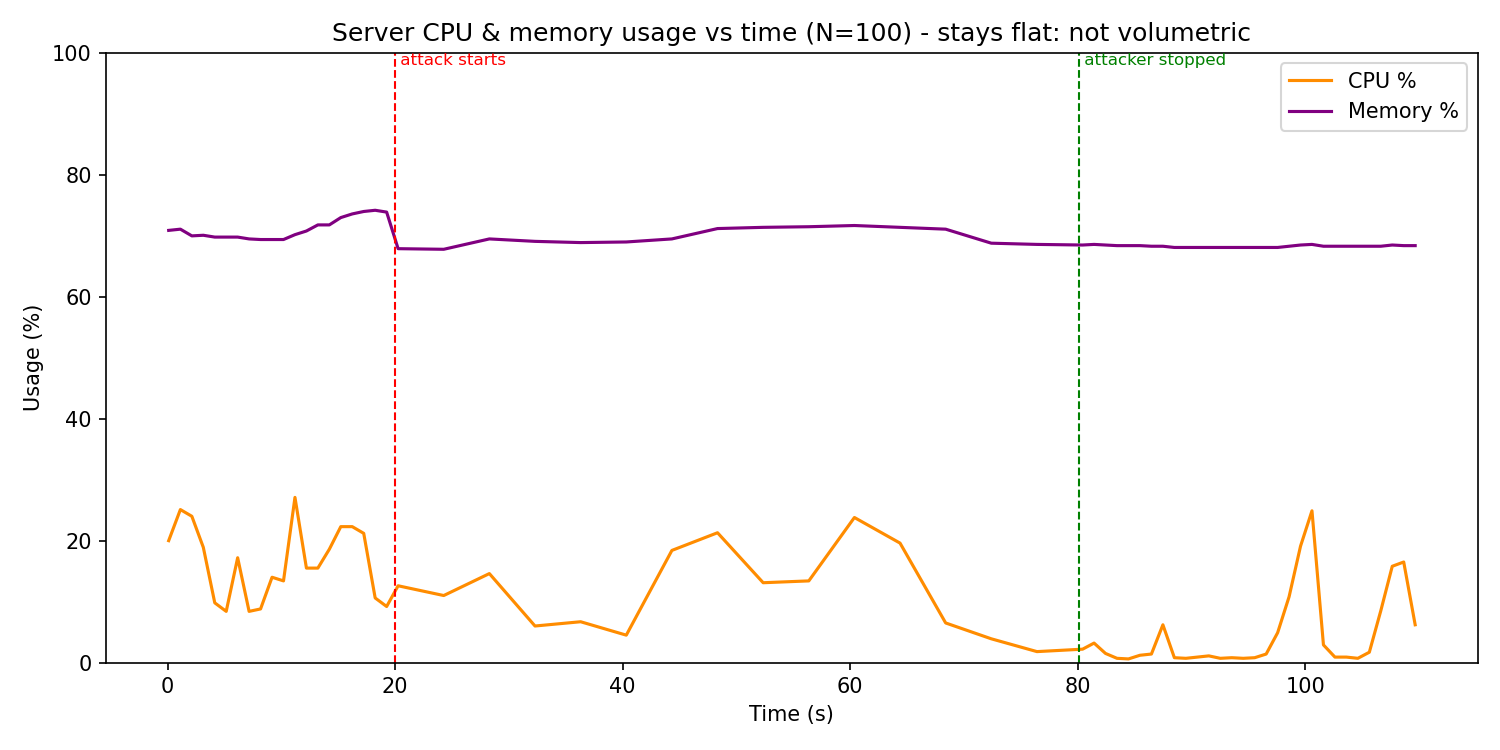
\includegraphics[width=0.85\textwidth]{../results/sweep_N100/2_cpu_mem.png}
\caption{Server CPU and memory usage during the $N=100$ attack. Usage
remains low throughout, showing that the server was not short on
computing power, it was short on available connection slots.}
\end{figure}

\section{The Defense}

\subsection{What Defense Was Applied}

Two complementary protective measures were put in place:

\begin{enumerate}
    \item \textbf{A cap on how long any single connection may take to
    finish sending its request.} If a connection does not complete its
    request within a bounded time, it is closed and its slot is freed,
    regardless of what the client does after that.
    \item \textbf{A limit on how many simultaneous connections a single
    source may hold open at once.} No matter how many connections one
    source attempts, only a small number of them are allowed through;
    the rest are refused outright before they can consume server
    capacity.
\end{enumerate}

Together, these measures bound how much of the server's total capacity
any one source, legitimate or malicious, can occupy at a time.

In practice, the first measure was implemented by enabling Apache's
request-timeout module with a header read window of 10 to 20 seconds
(and a minimum data rate of 500 bytes/second), so a connection sending
data too slowly is closed well before it could occupy a slot
indefinitely. The second measure was implemented as a firewall rule
that permits at most 10 simultaneous connections on port 80 from any
single source IP address, rejecting anything beyond that at the network
level before it ever reaches Apache.

\subsection{Was the Defense Successful?}

Yes. Table~\ref{tab:defense-results} shows the same measurements as
before, this time with the defense active.

\begin{table}[H]
\centering
\caption{Legitimate client outcomes during the attack window, defended server.}
\label{tab:defense-results}
\begin{tabular}{lllll}
\toprule
Attack size (N) & Client success rate & Avg.\ latency & Busy slots at peak & Result \\
\midrule
20  & 100\% & 0.05s & 12 / 30 & No denial \\
50  & 100\% & 0.01s & 11 / 30 & No denial \\
100 & 100\% & 0.01s & 11 / 30 & No denial \\
200 & 100\% & 0.00s & 10 / 30 & No denial \\
\bottomrule
\end{tabular}
\end{table}

With the defense active, the legitimate user's success rate stayed at
100\% and response times stayed near-instant at every attack size
tested, including sizes that had completely denied service before the
defense was applied.

\subsection{Why the Defense Was Successful}

The connection cap meant that, no matter how large the attacker's
intended attack size was, only a small handful of its connections ever
actually got through, the rest were rejected immediately. That small
number stayed far below the server's total capacity of 30 slots, so the
server always had plenty of room left for legitimate traffic. The
request-time cap provided a second layer of protection: even a
connection that did get through could only stall for a bounded amount
of time before being closed and its slot reclaimed. Because scaling the
attack size up further did not increase how many connections actually
reached the server, the defended results stay essentially flat across
every attack size tested; the defense's effect does not depend on how
big the attack is.

\subsection{Observed Output}

\begin{figure}[H]
\centering
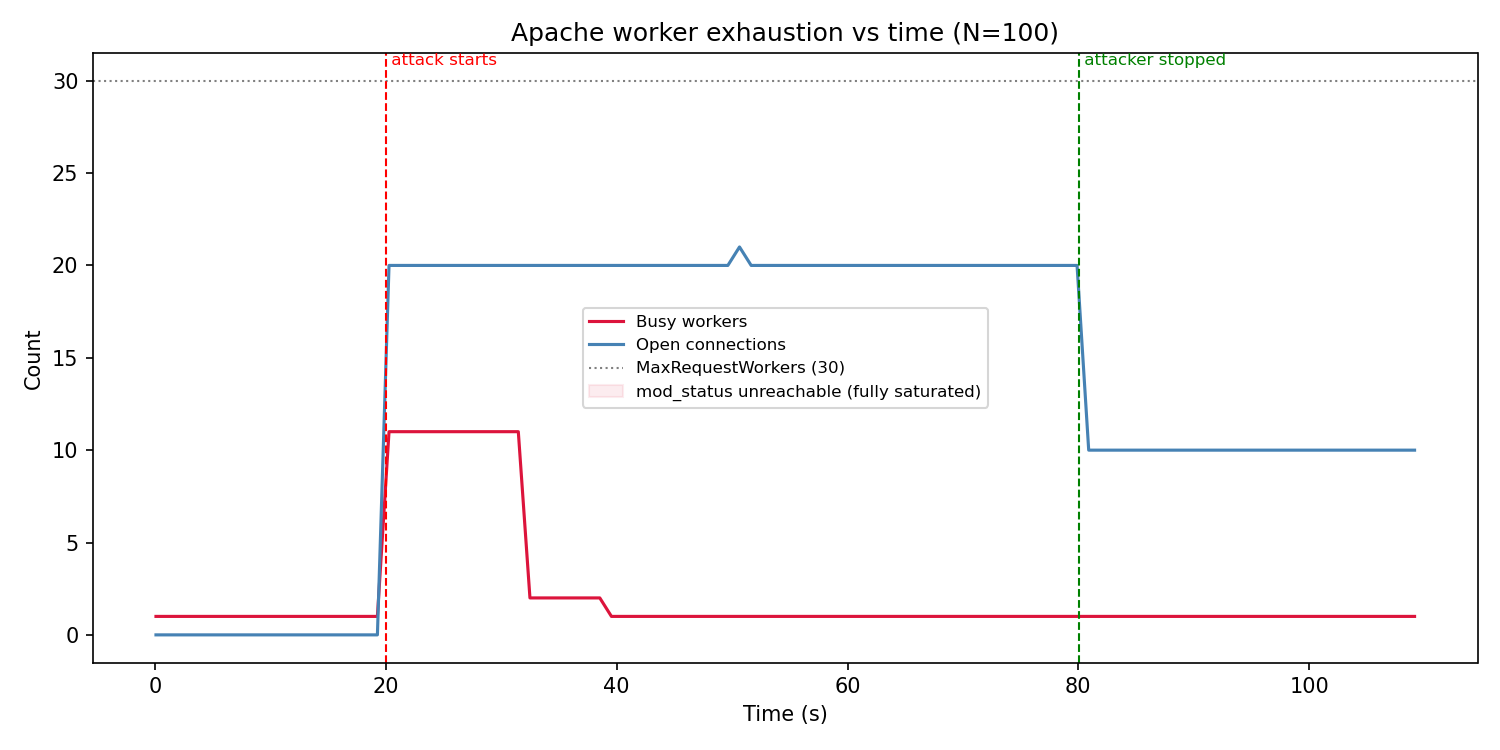
\includegraphics[width=0.85\textwidth]{../results_defended/sweep_N100/1_worker_saturation.png}
\caption{Busy connection slots over time during the $N=100$ attack, with
the defense active. Occupied slots stay low throughout, never
approaching the server's 30-slot limit.}
\end{figure}

\begin{figure}[H]
\centering
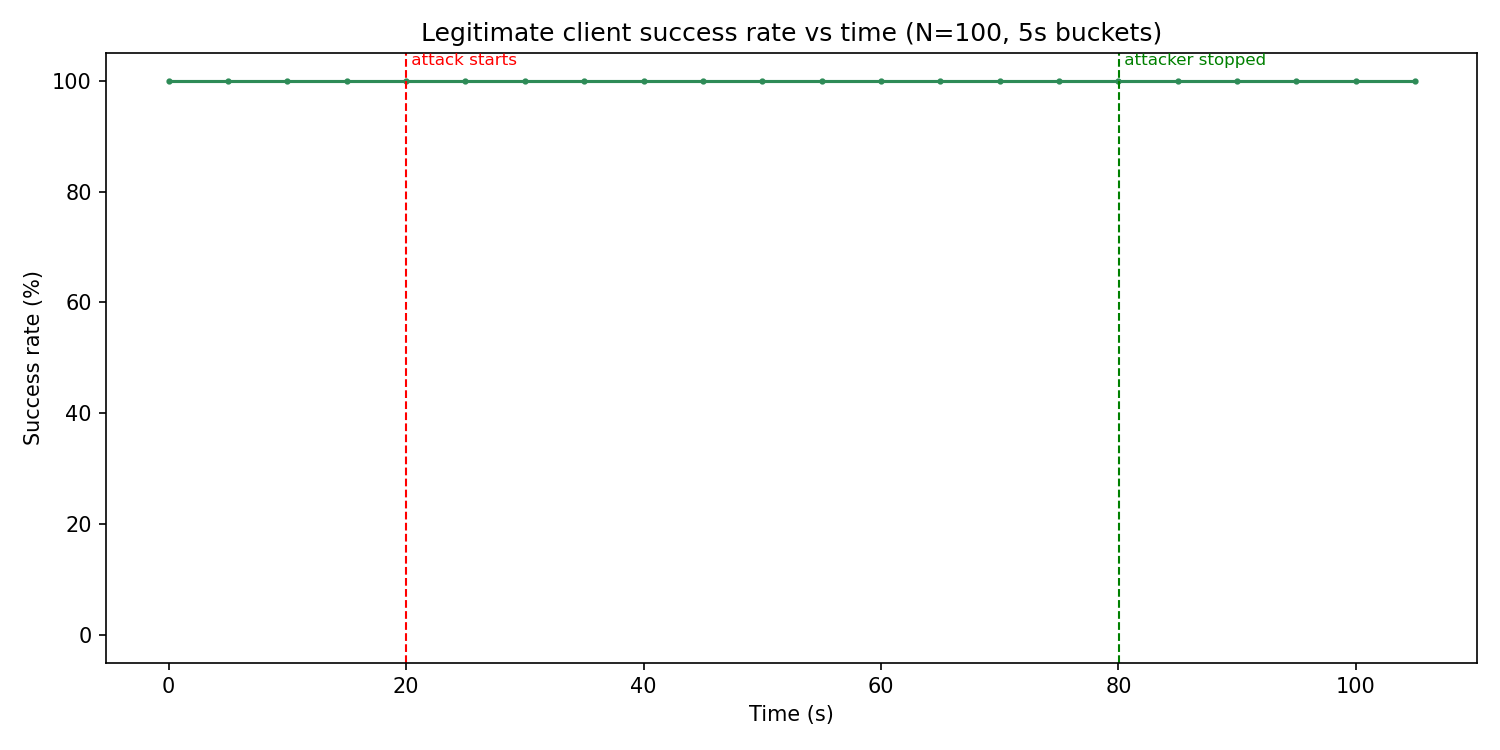
\includegraphics[width=0.85\textwidth]{../results_defended/sweep_N100/3_client_success_rate.png}
\caption{Legitimate client success rate over time during the $N=100$
attack, with the defense active. Success remains at 100\% throughout,
including during the attack window.}
\end{figure}

\begin{figure}[H]
\centering
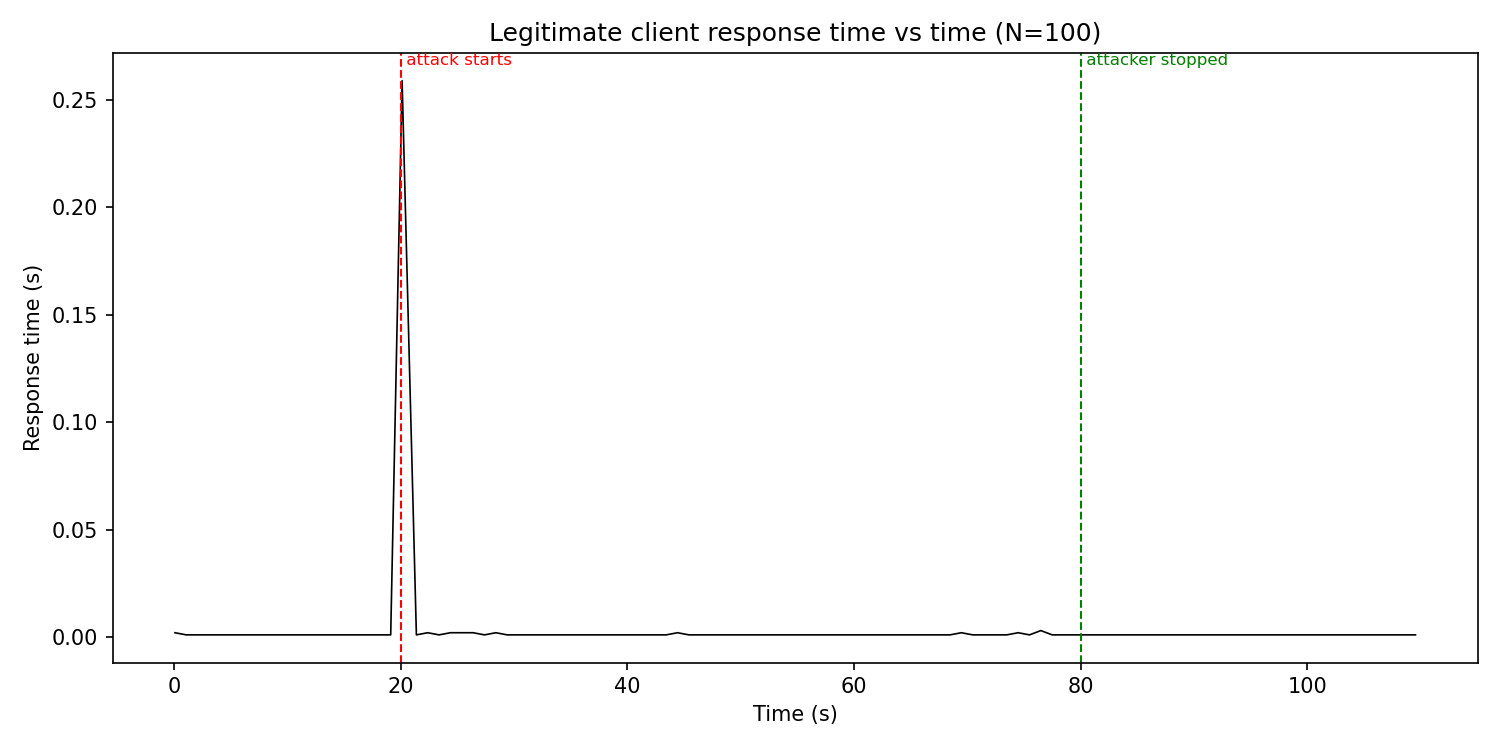
\includegraphics[width=0.85\textwidth]{../results_defended/sweep_N100/4_client_latency.png}
\caption{Legitimate client response time over time during the $N=100$
attack, with the defense active. Response times remain low and stable
throughout the attack window.}
\end{figure}

\begin{figure}[H]
\centering
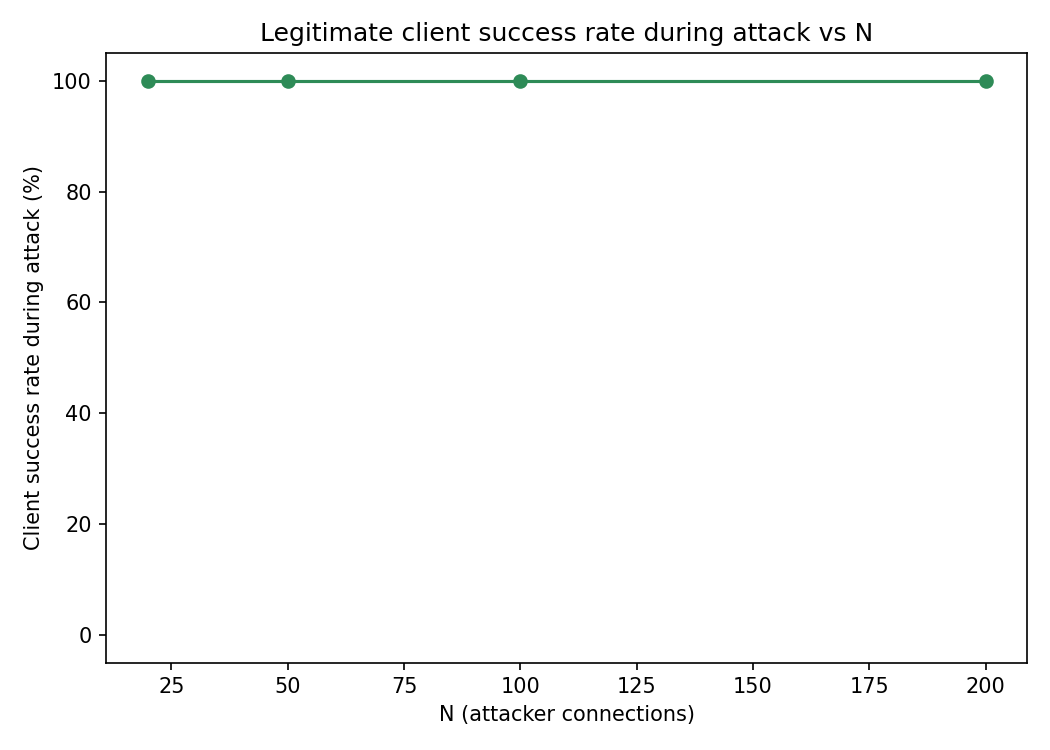
\includegraphics[width=0.6\textwidth]{../results_defended/sweep_comparison.png}
\caption{Legitimate client success rate across all tested attack sizes,
with the defense active. Success stays at 100\% regardless of attack
size, in contrast to the undefended results. (The time-to-saturation
panel shown for the undefended run is omitted here, since the server
never saturated at any tested attack size with the defense active.)}
\end{figure}

\section{Comparison}

Figure~\ref{fig:comparison} places the undefended and defended results
for the same attack size side by side. Before the defense, exceeding the
server's capacity threshold caused legitimate traffic to fail almost
entirely; after the defense, the same attack size had no visible effect
on legitimate traffic at all.

\begin{figure}[H]
\centering
\begin{minipage}{0.48\textwidth}
\centering
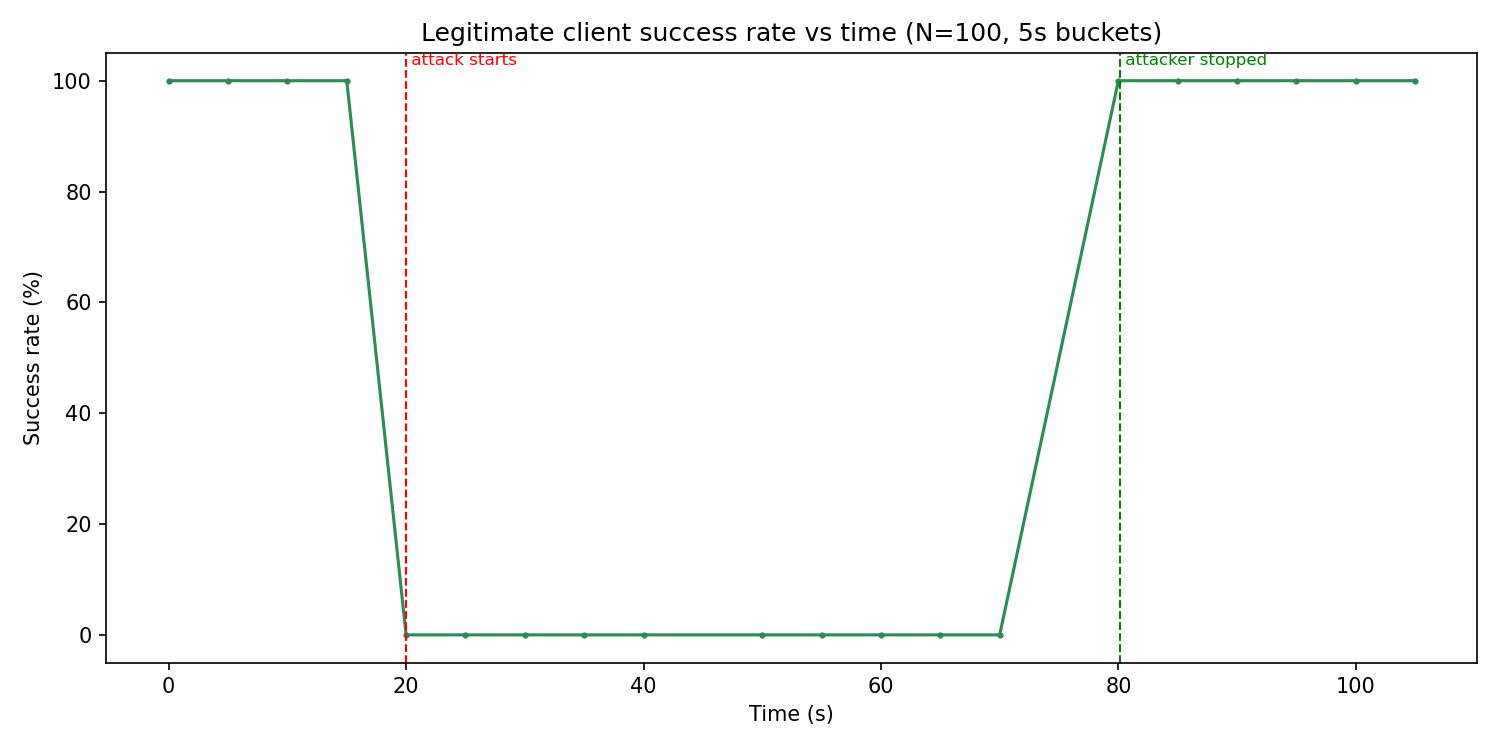
\includegraphics[width=\textwidth]{../results/sweep_N100/3_client_success_rate.png}
\caption*{Undefended, $N=100$}
\end{minipage}
\hfill
\begin{minipage}{0.48\textwidth}
\centering
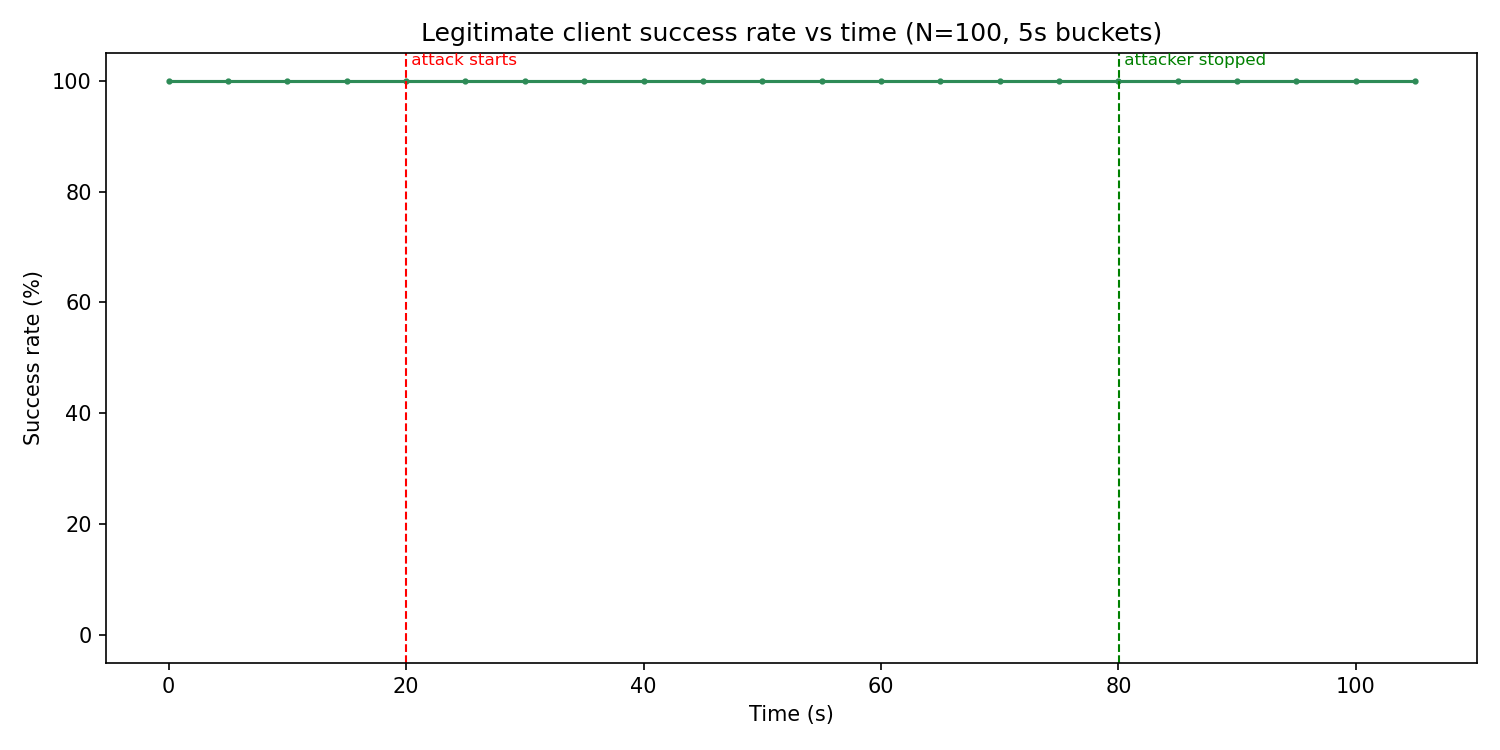
\includegraphics[width=\textwidth]{../results_defended/sweep_N100/3_client_success_rate.png}
\caption*{Defended, $N=100$}
\end{minipage}
\caption{Legitimate client success rate during the same attack size,
before and after the defense was applied.}
\label{fig:comparison}
\end{figure}

\section{Limitations}

\begin{itemize}
    \item The test was run on a single local machine rather than over a
    real network, so conditions such as multiple attacker locations,
    real network latency, and other traffic sharing the link were not
    present.
    \item The connection-limit defense depends on being able to tell the
    attacker apart from legitimate users by their source. Against an
    attack spread across many different sources at once, this specific
    measure becomes much harder to apply effectively, though the
    request-time cap still provides some protection regardless of
    source.
\end{itemize}

\section{Conclusion}

The attack succeeded once its size exceeded the server's spare capacity,
causing legitimate users to be denied service almost entirely. Applying
a combination of a per-connection time limit and a per-source connection
cap prevented any single source from consuming enough of the server's
capacity to cause that exhaustion, restoring normal service to
legitimate users even under attack sizes that had previously caused a
complete denial of service.

\end{document}
